\section{Pianificazione dei test}
	\subsection{Descrizione dei test}
		Vengono ora indicati i test di validazione, di sistema e di integrazione previsti. I test di unità saranno inseriti in un momento successivo. \\
		Poiché i test saranno applicati in uno stadio di lavoro successivo a quello attuale, lo stato dei singoli è indicato come \textbf{N.I.}: non implementati. \\
		Di ogni test verranno indicati la tipologia ed altri parametri come specificato dalla seguente sintassi:
		\begin{itemize}
					\item per i test di unità: \textbf{TU[Codice Test]};
					\item per i test di integrazione: \textbf{TI[Identificativo del componente]};
					\item per i test di sistema: \textbf{TS[Tipo Requisito][Codice Requisito]};
					\item per i test di validazione: \textbf{TV[Tipo Requisito][Codice Requisito]}.
		\end{itemize}
		In particolare:
		\begin{itemize}
			\item \textbf{Codice Requisito}: è il codice gerarchico univoco di ogni vincolo espresso in numero (esempio: 1.3.2);
			\item \textbf{Identificativo del componente}: corrisponde al componente i cui elementi sono integrati;
			\item \textbf{Tipo Requisito}: può assumere solo uno fra i seguenti valori:
			\begin{itemize}
				\item F: funzionale;
				\item Q: di qualità;
				\item P: prestazionale;
				\item V: di vincolo.
			\end{itemize}
		\end{itemize}
	\subsection{Modello a V}
			Per la pianificazione dei test si utilizzerà il Modello a V. Secondo questo modello il testing del software viene suddiviso in livelli differenti, i quali si concretizzano in un'esecuzione bottom-up che avanza sequenzialmente alle attività di codifica e di validazione. Ad ogni livello corrisponde un ciclo di uno specifico tipo di test, ed ogni test viene creato in base al relativo livello di progettazione.
			\begin{figure}[htp]
				\centering
				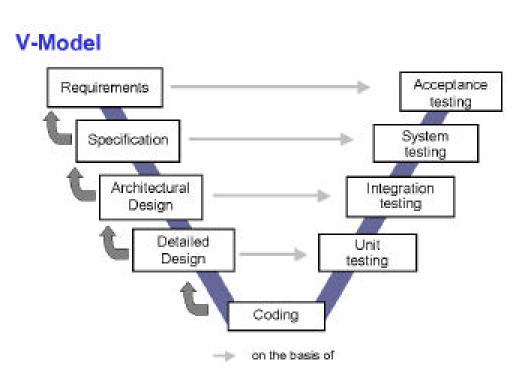
\includegraphics[width=0.5\textwidth]{img/V-model.jpg}
				\caption{Modello a V}
			\end{figure}
	\subsection{Test di validazione}
		I test di validazione servono per accertarsi che il prodotto realizzato sia conforme alle attese di \PROPONENTE. \\
		Per ognuno vengono indicati i passi necessari all'utente per testare i requisiti associati. Il tracciamento tra i test di validazione e i requisiti correlati viene riportato nel documento \ARdoc.
	\subsection{Test di sistema}
		I test di sistema servono per accertarsi che il comportamento dinamico del sistema rispetti i requisiti software individuati e descritti nel documento \ARdoc.
	\subsection{Test di integrazione}
		I test di integrazione servono per verificare che tutti i diversi componenti del sistema comunichino correttamente tra loro, e che vi sia all'interno del software il flusso di dati atteso. \\
		Verrà utilizzata una strategia di integrazione incrementale per poter sviluppare e verificare più componenti in parallelo. Questo metodo permette di dare priorità ai test relativi alle componenti che vengono ritenute più importanti e quindi sarà possibile partire dalle componenti che soddisfano i requisiti obbligatori fino ad integrarle con quelle che soddisfano i requisiti opzionali. Inoltre permette di restringere la ricerca dell'errore in caso di test fallito, perché molto probabilmente l'errore si trova nel nuovo componente o dalla sua interazione con il sistema corrente. Non si dovrà escludere il caso in cui il test fallisca perché la nuova istanza di test utilizza un campione di input non trattato in precedenza, portando così il sistema a generare l'errore. \\
		L'integrazione delle parti è bottom-up: innanzitutto verranno inserite le componenti con meno dipendenze funzionali e più funzionalità, cioè che corrispondono ai requisiti obbligatori. Di conseguenza queste componenti saranno testate molte volte in modo da ridurre la possibilità che il prodotto finale contenga difetti, e così si otterrà una versione funzionante nel minor tempo possibile. In seguito si risalirà l'albero delle dipendenze fino all'inserimento delle componenti di alto livello. \\
		Questo metodo è più oneroso rispetto ad altri in quanto richiede che venga generato del codice di supporto, sotto forma di driver e stub, che simuli le componenti mancanti, però permette una maggiore copertura perché testa ripetutamente le componenti più importanti.